\section{Purpose Definition}

% Persona block: #1 ID, #2 name, #3 differentiator, #4 technological resources, #5 needs, #6 purposes, #7 personal-information rows
\newcommand{\persona}[7]{%
\noindent\begin{minipage}[t]{0.66\linewidth}
\textbf{#1 -- #2}\\[2pt]
\textbf{Differentiator.} #3\\[2pt]
\textbf{Technological resources.} #4\\[2pt]
\textbf{Needs.} #5\\[2pt]
\textbf{Purposes.} #6
\end{minipage}\hfill
\begin{minipage}[t]{0.3\linewidth}
\small
\renewcommand{\arraystretch}{1.15}
\begin{tabular}[t]{|l|l|}
\hline
\multicolumn{2}{|c|}{\textbf{Personal information}} \\ \hline
#7
\hline
\end{tabular}
\end{minipage}
\vspace{10pt}

}

This section formalizes the informal purpose of Section~\ref{sec:informal-purpose}. Following the iTelos methodology, the purpose is first formalized through scenarios, personas and competency questions (CQs), from which the entity types (etypes), their properties and the ER model are derived; the information needed to satisfy it is then gathered. Every CQ traces back to at least one scenario and one persona, and every property is needed to answer at least one CQ.

\subsection{Purpose Formalization}

\subsubsection{Scenarios}
\label{sec:scenarios}
The scenarios describe, in the user's own voice, the situations in which the KG is used. Each one covers a different aspect of planning a hike.

\begin{description}
    \item[S1 -- A trail that suits me.] I would like to go hiking but I am not an expert and I do not understand the letters used to grade the trails. I want to say how much experience I have, whether I mind steep climbs and how much time I have, and be shown the trails that fit.
    \item[S2 -- Getting to the start.] I have chosen a trail and now I need to get there. If I drive, I need to know where the trail starts and where I can leave the car. If I do not have a car, I need to know which bus or train to take and at which stop to get off.
    \item[S3 -- Lunch on the way.] I will be out for several hours. I want to know whether there is a mountain hut or a restaurant along the trail where I can eat, or whether I have to pack my own lunch.
    \item[S4 -- What to wear and bring.] I do not know what I need for this trail. I want to be told which equipment its difficulty requires and how to dress, given the weather forecast for the day and how high the trail goes.
    \item[S5 -- Is it a good day for it?] It has rained a lot this week and there may still be snow higher up. Before I leave I want to know whether there has recently been heavy rain or snow near the trail, so that I can be careful or choose another one.
    \item[S6 -- Near a place I like.] I am staying near a lake and I want a trail that starts close to where I am, or close to a place I want to visit. I would also like to know if I can take a cable car up and walk mostly downhill.
\end{description}

\subsubsection{Personas}
\label{sec:personas}
The personas are the typical users acting within the scenarios. Sofia, an inexperienced hiker with a car, is the main persona: for her the KG has to provide complete, ready-to-use guidance.

\persona{P1}{Sofia}{Sofia is a 24-year-old Erasmus student who has been living in Trento since September. She has a car and wants to spend her Saturdays in the mountains, but she has hardly ever hiked and does not know the area or the trail difficulty scale. She does not like steep climbs.}{Smartphone, internet.}{Guidance, safety, autonomy.}{Sofia wants an easy trail without steep climbs and everything she needs to do it: where to park, how long it takes, whether to pack lunch, and what to wear and bring.}{ID & 1 \\ Age & 24 \\ Sex & F \\ Occupation & Student \\ Driver & yes \\ Education & Bachelor's \\}

\persona{P2}{Jonas}{Jonas is 26 and moved to Trento for work a few months ago. He is a beginner like Sofia, but he does not have a car and gets around by bus and train.}{Smartphone, internet.}{Accessibility, guidance, safety.}{Jonas wants easy trails that he can reach by public transport, knowing which bus or train to take and at which stop to get off, and what to wear and bring.}{ID & 2 \\ Age & 26 \\ Sex & M \\ Occupation & Employee \\ Driver & no \\ Education & Master's \\}

\persona{P3}{Giulia}{Giulia is 38 and lives in Rovereto with her partner and their two children, aged five and eight. They go out by car at weekends; the children cannot walk for long and need a proper stop for lunch.}{Smartphone, internet, PC.}{Convenience, safety, a relaxed family day.}{Giulia wants a short, easy trail with a hut for lunch and parking close to the start, or a lift that saves the climb.}{ID & 3 \\ Age & 38 \\ Sex & F \\ Occupation & Teacher \\ Driver & yes \\ Education & Master's \\}

\persona{P4}{Marco}{Marco is 45, was born in Trentino and has been hiking since he was a child. He looks for long, demanding routes and decides himself how much ascent and how many hours he wants.}{Smartphone, internet, GPS watch.}{Challenge, autonomy, reliable information on conditions.}{Marco wants trails at his level that he can compare by ascent and duration, and he wants to know about recent snow and rain and the equipment required before he sets out.}{ID & 4 \\ Age & 45 \\ Sex & M \\ Occupation & Engineer \\ Driver & yes \\ Education & Master's \\}

\persona{P5}{Luca}{Luca is 31 and works at a tourist information office on Lake Garda. Every day visitors of all levels ask him where they can hike nearby.}{PC, internet, smartphone.}{Quick, reliable answers for other people.}{Luca wants to recommend trails near the places tourists visit, suited to each visitor, and to warn them when recent weather makes a trail unsuitable.}{ID & 5 \\ Age & 31 \\ Sex & M \\ Occupation & Tourist office clerk \\ Driver & yes \\ Education & Bachelor's \\}

\subsubsection{Competency Questions}
\label{sec:cqs}
Table~\ref{tab:cqs} lists the CQs with the scenarios and personas they come from and the etypes needed to answer them, grouped by focus (Section~\ref{sec:concepts}). The CQs are phrased as the personas would ask them. ``This trail'' in CQ5--CQ11 refers to a trail selected from the answers to CQ1--CQ4, ``today'' stands for the day of the hike, and CQ12 combines the others into the main use case of the KG.

\begin{table}[htbp]
\centering\footnotesize
\renewcommand{\arraystretch}{1.25}
\begin{tabular}{|>{\raggedright\arraybackslash}p{0.8cm}|>{\raggedright\arraybackslash}p{0.9cm}|>{\raggedright\arraybackslash}p{1.1cm}|>{\raggedright\arraybackslash}p{4.4cm}|>{\raggedright\arraybackslash}p{2.3cm}|>{\raggedright\arraybackslash}p{2.6cm}|>{\raggedright\arraybackslash}p{2.3cm}|}
\hline
\textbf{ID} & \textbf{Scen.} & \textbf{Pers.} & \textbf{Competency question} & \textbf{Common etypes} & \textbf{Core etypes} & \textbf{Contextual etypes} \\ \hline
CQ1 & S1 & P1, P2, P3 & I'm an inexperienced hiker and don't like steep climbs -- which trails suit me? & & Trail, DifficultyLevel, ExperienceLevel, InclineCategory & \\ \hline
CQ2 & S1 & P4 & I'm an experienced hiker -- which trails match my level, and how do they compare in ascent and duration? & & Trail, DifficultyLevel, ExperienceLevel & \\ \hline
CQ3 & S6 & P1--P5 & Which suitable trails start near me, or near a place I want to visit? & Municipality, PointOfInterest & Trail, Trailhead & \\ \hline
CQ4 & S6 & P1, P3 & Can I take a cable car or lift up and then hike mostly downhill? & Lift & Trail, Trailhead & \\ \hline
CQ5 & S1 & P1--P5 & How long does this trail take, how long is it, and what are its ascent and descent? & & Trail & \\ \hline
CQ6 & S3 & P1, P3, P4 & Is there a hut or restaurant on the way, or should I pack lunch? & PointOfInterest & Trail & \\ \hline
CQ7 & S2 & P1, P3, P4 & I have a car -- where does the trail start and where can I park? & CarPark & Trail, Trailhead & \\ \hline
CQ8 & S2 & P2 & I don't have a car -- how do I get to the trail by public transport (which bus or train, and which stop)? & TransportStop, TransitLine & Trail, Trailhead & \\ \hline
CQ9 & S4 & P1--P5 & What equipment do I need for this trail? & & Trail, DifficultyLevel, Equipment & \\ \hline
CQ10 & S4 & P1--P5 & How should I dress for this trail today, given the forecast and the altitude? & Municipality & Trail, Trailhead, Equipment & WeatherForecast, HikingCondition \\ \hline
CQ11 & S5 & P1--P5 & Has there been heavy rain or snow near this trail recently -- should I be careful? & & Trail & WeatherStation, DailyObservation, HikingCondition \\ \hline
CQ12 & S1--S5 & P1 & I'm inexperienced, have a car and don't like steep trails -- what are my options today, how long do they take, where do I park, do I need lunch, and what should I wear and bring? & CarPark, PointOfInterest, Municipality & Trail, Trailhead, DifficultyLevel, ExperienceLevel, InclineCategory, Equipment & WeatherStation, DailyObservation, WeatherForecast, HikingCondition \\ \hline
\end{tabular}
\caption{Competency questions with their scenarios, personas and the etypes they require.}
\label{tab:cqs}
\end{table}

\subsubsection{Concepts Identification}
\label{sec:concepts}
From the CQs we extracted the concepts identifying the etypes and their properties. Each of them is assigned a \textbf{focus}, which states how crucial it is for the purpose: \emph{core} etypes are specific to the purpose, \emph{common} etypes are general ones also found in many other domains, and \emph{contextual} etypes are very specific to this purpose. The complete Purpose Formalization sheet, with the focus of every single property, is available in the project repository (\texttt{Phase 1 - Purpose Definition/PFsheet.xlsx}).

\noindent Attributes are divided into \emph{identifying} attributes, which give each entity a unique identity and are taken from how the records are structured in the datasets, and \emph{descriptive} attributes, which are the facts the CQs ask about. The identifying attributes listed here are those expected from the data sources and will be confirmed during information gathering.

\noindent An important design choice is that the KG itself translates the user's words into formal criteria. A beginner does not need to know what ``T'' or ``E'' means: ExperienceLevel is linked to the difficulty levels that suit it, and InclineCategory turns ``I don't like steep climbs'' into a threshold on ascent per kilometre. Likewise, the rules that decide which extra equipment is needed under given conditions (HikingCondition) are stored as data in the KG rather than hidden in query code, so that they can be inspected and changed.

\begin{table}[htbp]
\centering\footnotesize
\renewcommand{\arraystretch}{1.25}
\begin{tabular}{|>{\raggedright\arraybackslash}p{2.5cm}|>{\raggedright\arraybackslash}p{1.6cm}|>{\raggedright\arraybackslash}p{3.9cm}|>{\raggedright\arraybackslash}p{2.9cm}|>{\raggedright\arraybackslash}p{4.0cm}|}
\hline
\textbf{Etype} & \textbf{Focus} & \textbf{Description} & \textbf{Identifying attributes} & \textbf{Descriptive attributes} \\ \hline
Trail & Core & An official SAT hiking trail. & trailId (SAT number), osmRelationId & name, lengthKm, durationMin, ascentM, descentM, maxAltitudeM \\ \hline
Trailhead & Core & A point where a trail starts or ends. & trailheadId & name, latitude, longitude, altitudeM \\ \hline
DifficultyLevel & Core & A level of the CAI/SAT difficulty scale. & code (T, E, EE, EEA) & name, description \\ \hline
ExperienceLevel & Core & The experience of a hiker, linked to the difficulty levels that suit it. & name & description \\ \hline
InclineCategory & Core & How steep a trail is. & name (gentle, moderate, steep) & maxAscentM, maxAscentPerKm \\ \hline
Equipment & Core & An item of gear or clothing. & name & category (gear, clothing), description, source \\ \hline
Municipality & Common & A municipality of Trentino; forecasts refer to municipalities. & istatCode & name, altitudeM \\ \hline
CarPark & Common & A public car park. & carParkId & name, latitude, longitude, capacity, fee \\ \hline
TransportStop & Common & A bus stop or train station. & stopId & name, latitude, longitude \\ \hline
TransitLine & Common & A bus or train route (e.g.\ bus number 5). & routeId & shortName, longName, mode (bus, rail) \\ \hline
PointOfInterest & Common & A place along or near a trail: mountain hut, restaurant, lake, peak, castle, viewpoint. & poiId & name, poiType, latitude, longitude, altitudeM, openingHours \\ \hline
Lift & Common & A cable car, gondola or chairlift. & liftId & name, liftType, bottomAltitudeM, topAltitudeM, topLatitude, topLongitude \\ \hline
WeatherStation & Contextual & A Meteotrentino measuring station: a weather station or a snow measuring site. & stationCode & name, stationType (weather, snow), latitude, longitude, altitudeM \\ \hline
DailyObservation & Contextual & The measurements of one station on one day. & station and date & precipitationMm, tempMinC, tempMaxC, snowDepthCm, freshSnowCm \\ \hline
WeatherForecast & Contextual & The forecast for a municipality on a given day. & municipality, forecastDate and issueDate & tempMinC, tempMaxC, precipProbability, description \\ \hline
HikingCondition & Contextual & A rule defining a condition relevant to hikers (e.g.\ recent heavy rain, snow, cold at altitude). & name & variable, operator, threshold, windowDays \\ \hline
\end{tabular}
\caption{Etypes with their focus and their identifying and descriptive attributes.}
\label{tab:etypes}
\end{table}

\noindent Table~\ref{tab:relationships} lists the relationships (object properties) between the etypes and the CQs that require them.

\begin{table}[h!]
\centering
\small
\renewcommand{\arraystretch}{1.25}
\begin{tabularx}{\linewidth}{|>{\raggedright\arraybackslash}p{3.8cm}|>{\raggedright\arraybackslash}p{5.6cm}|>{\raggedright\arraybackslash}X|}
\hline
\textbf{Relationship} & \textbf{Domain $\rightarrow$ Range} & \textbf{Required by} \\ \hline
hasDifficulty & Trail $\rightarrow$ DifficultyLevel & CQ1, CQ2, CQ9, CQ12 \\ \hline
hasInclineCategory & Trail $\rightarrow$ InclineCategory & CQ1, CQ12 \\ \hline
suitableFor & ExperienceLevel $\rightarrow$ DifficultyLevel & CQ1, CQ2, CQ12 \\ \hline
startsAt, endsAt & Trail $\rightarrow$ Trailhead & CQ3, CQ4, CQ7, CQ8, CQ12 \\ \hline
passesNear & Trail $\rightarrow$ PointOfInterest & CQ3, CQ6, CQ12 \\ \hline
locatedIn & Trailhead $\rightarrow$ Municipality & CQ3, CQ10 \\ \hline
nearCarPark & Trailhead $\rightarrow$ CarPark & CQ7, CQ12 \\ \hline
nearStop & Trailhead $\rightarrow$ TransportStop & CQ8 \\ \hline
servedBy & TransportStop $\rightarrow$ TransitLine & CQ8 \\ \hline
topStationNear & Lift $\rightarrow$ Trailhead & CQ4 \\ \hline
nearestWeatherStation, nearestSnowStation & Trail $\rightarrow$ WeatherStation & CQ11, CQ12 \\ \hline
observedAt & DailyObservation $\rightarrow$ WeatherStation & CQ11, CQ12 \\ \hline
forecastFor & WeatherForecast $\rightarrow$ Municipality & CQ10, CQ12 \\ \hline
requiresEquipment & DifficultyLevel $\rightarrow$ Equipment & CQ9, CQ12 \\ \hline
recommendsEquipment & HikingCondition $\rightarrow$ Equipment & CQ10, CQ12 \\ \hline
\end{tabularx}
\caption{Relationships and the CQs that require them.}
\label{tab:relationships}
\end{table}

\subsubsection{ER Model}
\label{sec:er}
Figure~\ref{fig:er} shows the ER model built from the etypes and relationships above. It contains 16 etypes and 17 relationships; colours distinguish the focus of the etypes.

\begin{sidewaysfigure}
    \centering
    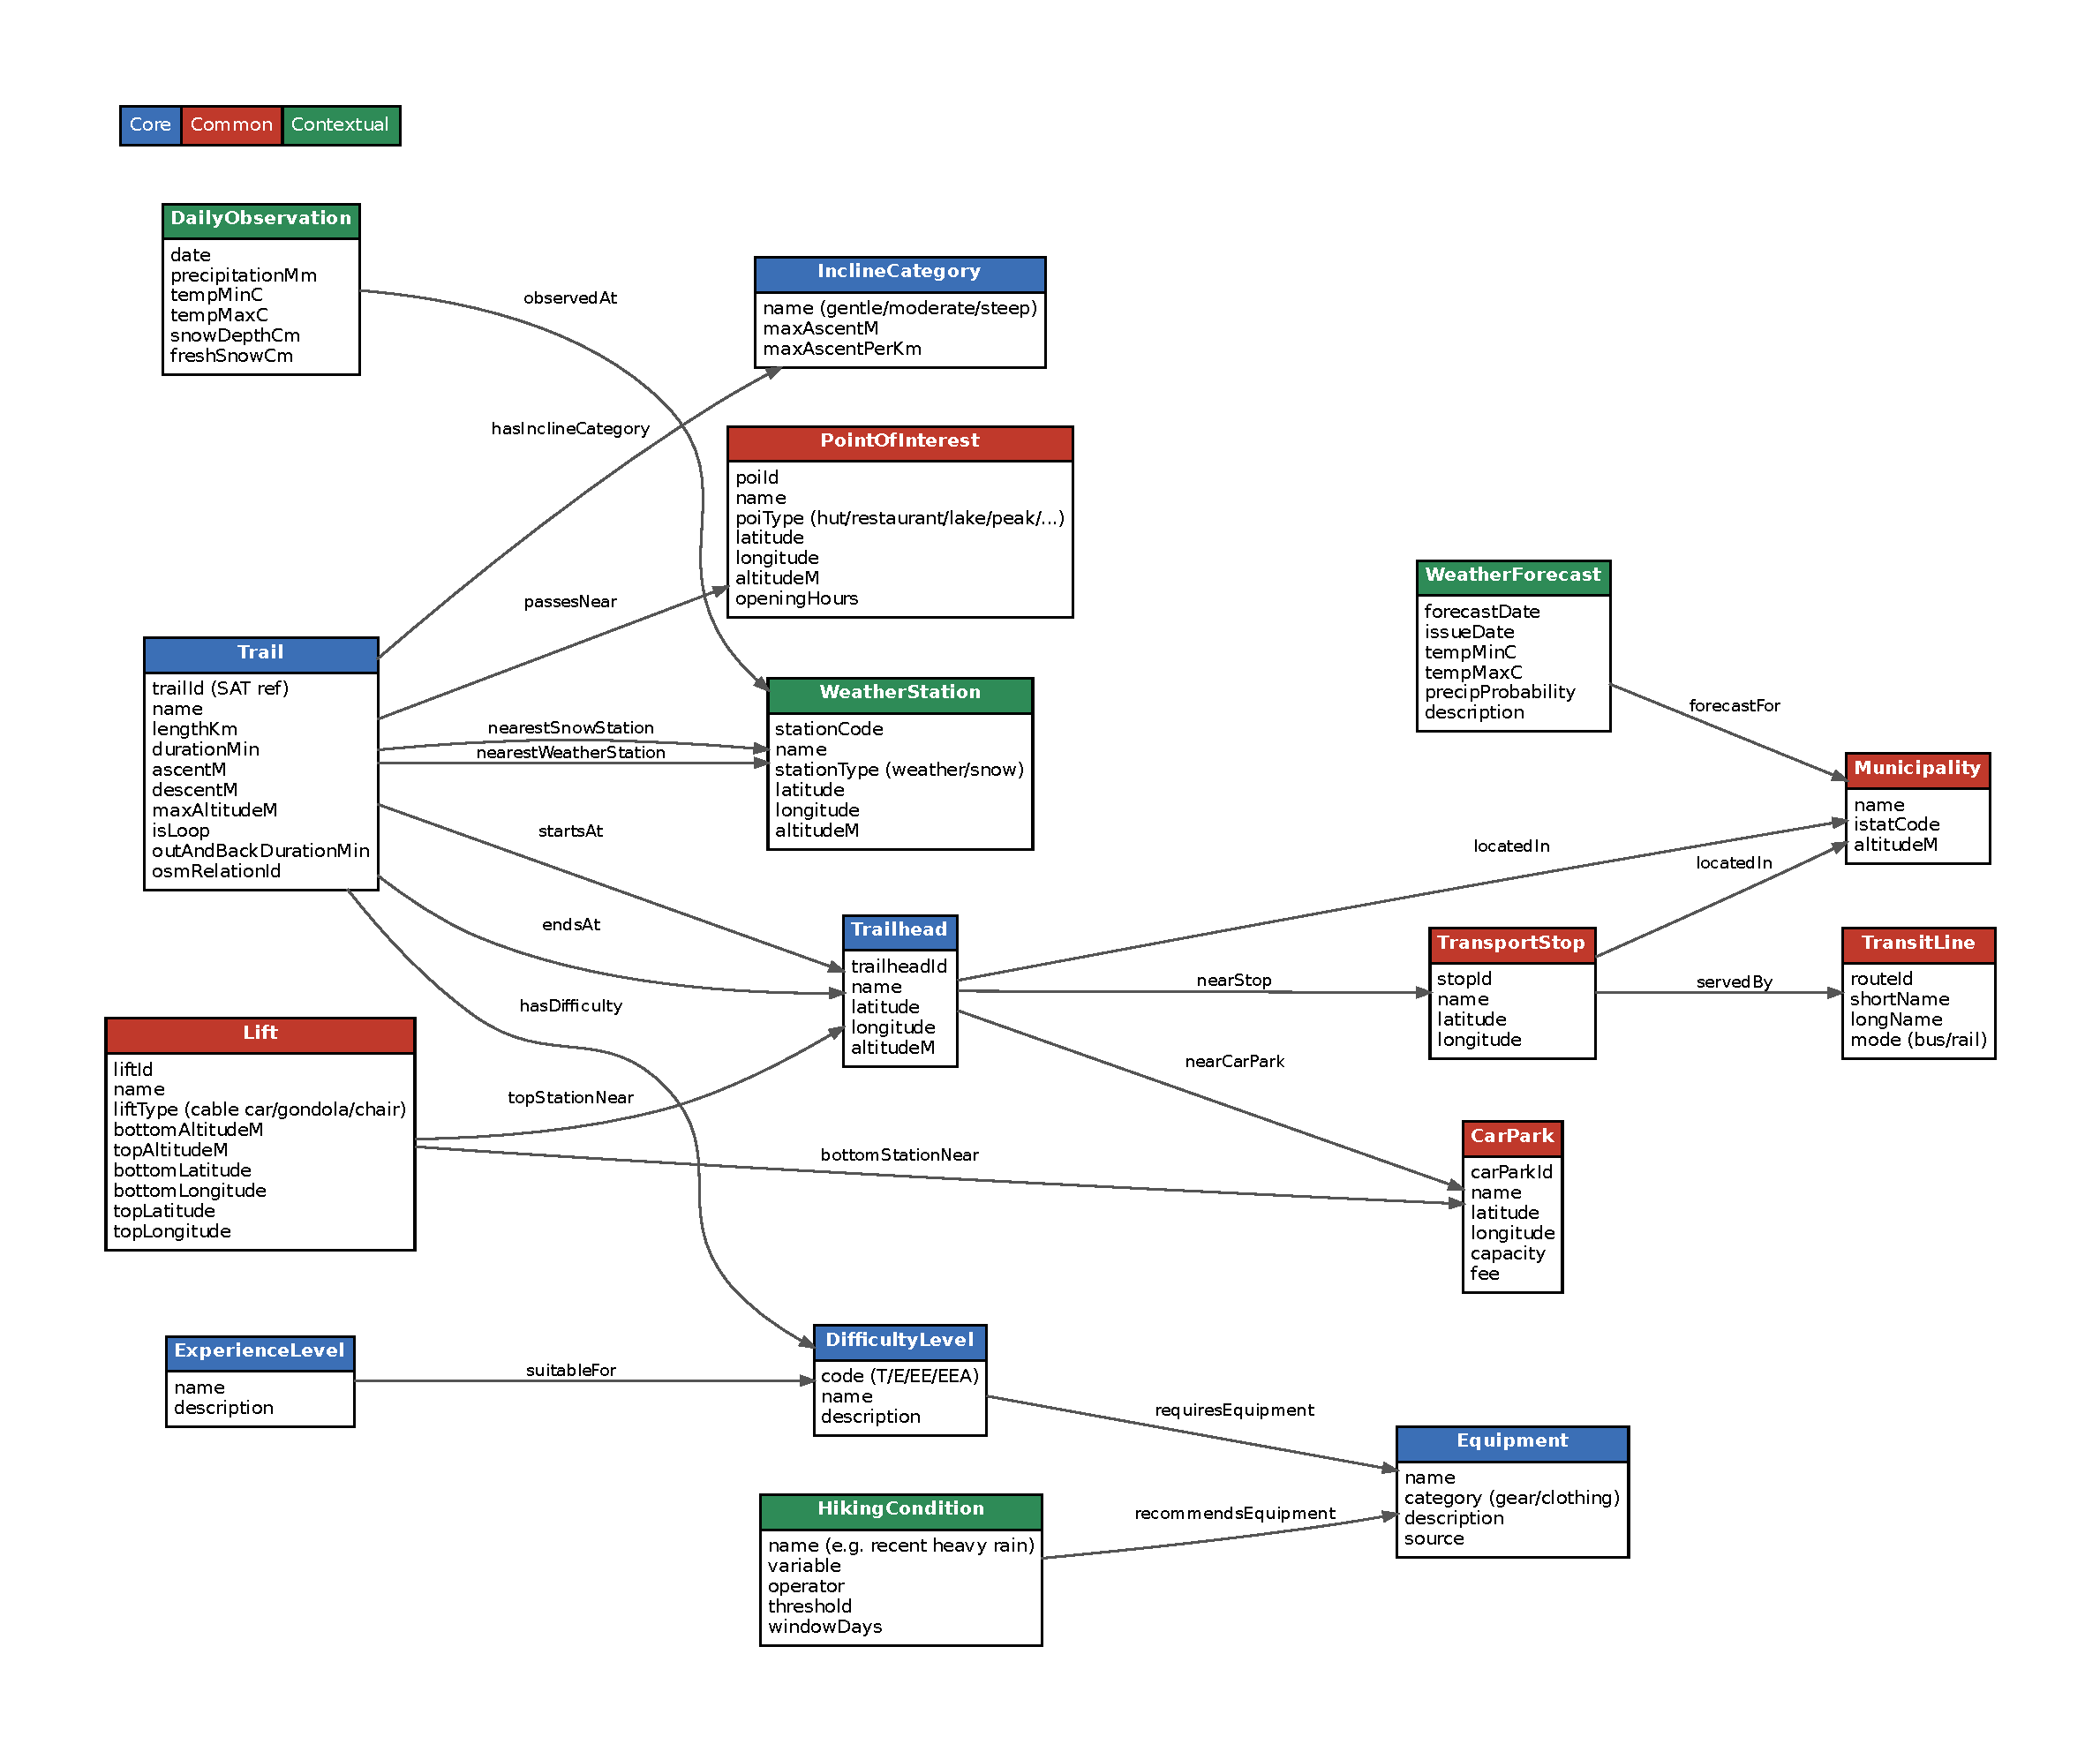
\includegraphics[width=\linewidth,height=0.85\textheight,keepaspectratio]{er_diagram}
    \caption{ER model of the Trentino Hikes KG. Blue: core etypes; red: common etypes; green: contextual etypes.}
    \label{fig:er}
\end{sidewaysfigure}

\noindent The main design choices, with their strong and weak points, are the following.
\begin{itemize}
    \item \textbf{User language as knowledge.} ExperienceLevel, InclineCategory and HikingCondition encode how a user's words map to formal criteria. \emph{Strong point}: beginners can query the KG without knowing the CAI/SAT scale, and the rules are explicit and reusable. \emph{Weak point}: thresholds such as what counts as ``steep'' or ``heavy rain'' are a team decision based on hiking guidelines and have to be documented as such.
    \item \textbf{Computed proximity relationships.} passesNear, nearCarPark, nearStop and topStationNear are not expected to exist in any dataset and would be computed from coordinates, with draft distances of 200\,m for points of interest along a trail, 500\,m for car parks and public transport stops from a trailhead, and 300\,m for the top station of a lift. Whether this is feasible, and with which distances, is decided once the data has been examined. \emph{Weak point}: straight-line distance does not account for terrain or access.
    \item \textbf{Nearest station as a proxy for conditions.} Rain and snow on a trail are estimated from the nearest weather station and the nearest snow measuring site at a similar altitude. \emph{Weak point}: stations can be several kilometres away from the trail.
    \item \textbf{One etype for all stations.} Weather stations and snow measuring sites share the same structure, so they are modelled as one etype with a stationType attribute, which keeps the model and the queries simpler.
    \item \textbf{One etype for all points of interest.} Huts, restaurants and attractions are modelled as PointOfInterest with a poiType attribute, so that the same relationship serves both the food question (CQ6) and the attractions question (CQ3). \emph{Alternative}: subclasses of PointOfInterest (e.g.\ MountainHut, Restaurant), which are better-behaved but less flexible. The choice is made once the data has been examined.
    \item \textbf{Representation of the forecast.} WeatherForecast is modelled as an etype of its own, identified by municipality, forecast date and issue date. How forecasts are best stored depends on the format in which they are published and is revisited during information gathering.
    \item \textbf{Model size.} With 12 CQs and 16 etypes the model is larger than the example projects of previous years. Each etype is required by at least one CQ (Table~\ref{tab:cqs}); whether the scope is kept or reduced is decided after the data sources have been examined.
\end{itemize}

% =====================================================================
% TODO: Information Gathering (next step of the project)
% Template structure to follow:
%   KG/KnowDive data sources  -> knowledge layer / data layer
%   External data sources     -> knowledge layer / data layer
%   each with: sources description, resources collection (and scraping),
%   classification over common, core and contextual
% =====================================================================
\subsection{Information Gathering}
\label{sec:info-gathering}
\textit{To be completed.}

\subsection{Qualitative Evaluation}
\label{sec:purpose-eval}
\textit{To be completed after information gathering.} So far the purpose has evolved as follows.
\begin{itemize}
    \item \textbf{Scenarios}: 5 scenarios were initially considered. Travel by car or public transport, gear and clothing, and taking a lift were added, giving 6 scenarios.
    \item \textbf{Personas}: 4 personas were initially considered. A persona without a car (Jonas) was added, giving 5 personas, with Sofia, an inexperienced hiker with a car, as the main persona.
    \item \textbf{CQs}: a first draft of 15 CQs was written in technical terms (e.g.\ ``trails of difficulty T or E''). Since the main users are inexperienced hikers who do not know the CAI/SAT scale, the CQs were rewritten in the users' own words and merged into 12, and the translation from user language to formal criteria was moved into the KG (ExperienceLevel, InclineCategory, HikingCondition).
    \item \textbf{Time scope}: a presentation scenario with a reference date in the summer hiking season was added, because the project runs in November--December, when most lifts and huts are closed.
\end{itemize}

\noindent \textit{Remarks on LLM usage and the phase-specific LLM questionnaire (Appendix A): to be completed.}
